\section{Auswertung}
\label{sec:Auswertung}
\subsection{Bestimmung der Zeitkonstanten RC mit der Entladekurve des Kondensators}
\label{sec:RC}
Zur Bestimmung der Zeitkonstanten RC werden aus der Entladekurve in Abbildung \ref{fig:plotrc} die Werte für $U_\text{C}$ abgelesen.
$U_\text{0}$ wurde bestimmt zu $U_\text{0}=\SI{6.04}{\volt}$.
Die abgelesenen Daten finden sich in Tabelle \ref{tab:taba}.
Durch Umformung wird Formel \eqref{eqn:aufladung} zu
\begin{equation}
	\label{eqn:ausgleich1}
	\ln\left(\frac{U_\text{C}}{U_\text{0}}\right)=-\frac{1}{RC}t \,\,\,\, (y = -m \cdot t).
\end{equation}
Zur Bestimmung der Zeitkonstanten $RC$ wird nun $\ln\left(\frac{U_\text{C}}{U_\text{0}}\right)$ gegen die Zeit $t$ aufgetragen.
Aus den Parametern der Regressionsgeraden nach Gleichung \eqref{eqn:ausgleich1} ergibt sich nun die berechnete Zeitkonstante zu

\begin{equation*}
	\centering
	RC = a = (0.48 \pm 0.03) \cdot 10^{-3} \si{\second} .
\end{equation*}
\begin{equation*}
	\centering
	b = (0.17 \pm 0.13)
\end{equation*}
\begin{table}
	\caption{Messdaten zur Bestimmung der Zeitkonstanten $RC$.}
	\label{tab:taba}
	\centering
	\begin{tabular}{ccc}
		\toprule
		$U_\text{C}$/$\si{\volt}$ & $\ln{(\frac{U_\text{C}}{U_\text{0}})}$ & $t$ /$10^{-3}\si{\second}$ \\
		\midrule
		6.04                      & 0.0000                                 & 0.00                       \\
		4.04                      & -0.4022                                & 0.25                       \\
		2.76                      & -0.7832                                & 0.50                       \\
		1.80                      & -1.2106                                & 0.75                       \\
		1.08                      & -1.7214                                & 1.00                       \\
		0.56                      & -2.3782                                & 1.25                       \\
		0.24                      & -3.2255                                & 1.50                       \\                    \\
		\bottomrule
	\end{tabular}
\end{table}
Die Messdaten sowie die berechnete lineare Regression befinden sich in Abbildung \ref{fig:plota}.
\begin{figure}
	\centering
	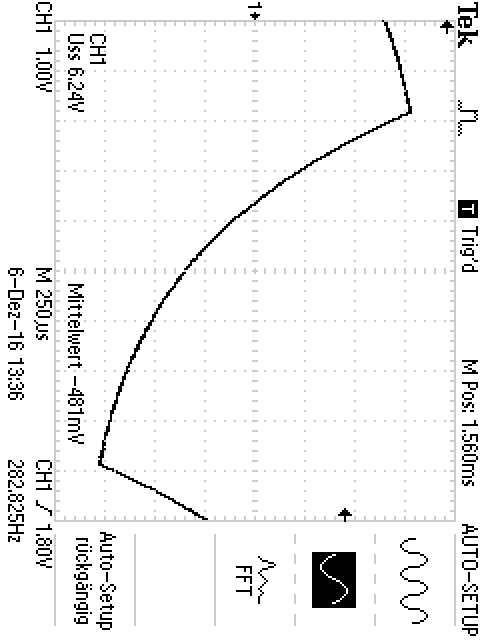
\includegraphics[angle=90]{bilder/F0000TEK.JPG}
	\caption{Aufgabenteil a: Entladekurve des Kondensators zur Bestimmung der Zeitkonstanten $RC$.}
	\label{fig:plotrc}
\end{figure}

\begin{figure}
	\centering
	\includegraphics{build/test.pdf}
	\caption{Lineare Regression zur Bestimmung der Zeitkonstanten $RC$.}
	\label{fig:plota}
\end{figure}

%%%%%%%%%%%%%%%%%%%%%%%%%%%%%%%%%%%%%%%%%%%%%%%%%%%%%%%%%%%%%%%%%%%%%%%%%%%%%%%%%%%%%%%%%%%
\subsection{Bestimmung der Zeitkonstanten RC über die Frequenzabhängigkeit der Amplitude.}
Die Zeitkonstante $RC$ soll nun erneut bestimmt werden, indem die Frequenzabhängigkeit der Amplitude $A(\omega)$ der Spannung $U_\text{C}$ am Kondensator untersucht wird.
Dazu wird $\frac{A(\omega)}{U_\text{0}}$ in Abhängigkeit zur Frequenz $\omega$ aufgetragen. Die verwendeten Daten befinden sich in Tabelle \ref{tab:tab2}.
$U_{\mathrm{0}}$ betrug hierbei $6.04 \,\si{\volt}$.
Eine Regression mit Gleichung \eqref{eqn:amplitude} liefert für die Zeitkonstante :

\begin{equation*}
	\centering
	RC = a =(6.3 \pm 1.5)\cdot 10^{-3} \si{\second} .
\end{equation*}
Mit Phyton und Scypi wurde hierfür die Funktion

\begin{equation*}
	f(\omega)=\frac{1}{\sqrt{1 +\omega^2 a^2}}
\end{equation*}
nach $\omega$ für den Parameter $a$ gefittet.
Werden die ersten vier Messpunkte ausgenommen, ergibt sich ein etwas kleinerer Fehler:

\begin{equation*}
	\centering
	RC = a =(6.2 \pm 0.5)\cdot 10^{-3} \si{\second} .
\end{equation*}
Somit haben die ersten Messpunkte nahezu keine Auswirkung auf das berechnete $RC$, obwohl sie sehr stark von der Regression abweichen, sie beeinflussen lediglich den Fehler der Zeitkonstanten.
%hoffe das reicht ihr
\begin{table}
	\caption{Messdaten zur Bestimmung der Zeitkonstanten $RC$ über die Frequenzabhängigkeit der Amplitude $A(\omega)$.}
	\label{tab:tab2}
	\centering
	\begin{tabular} {ccc}
		\toprule
		$A(\omega)$/ $\si{\volt}$ & $\frac{A(\omega)}{U_\text{0}}$ & $\omega$/$\si{\Hz}$ \\
		\midrule
		2.80                      & 0.46                           & 4.2                 \\
		4.40                      & 0.73                           & 10.0                \\
		4.88                      & 0.81                           & 15.0                \\
		5.04                      & 0.83                           & 20.0                \\
		5.20                      & 0.86                           & 35.0                \\
		5.12                      & 0.85                           & 60.0                \\
		4.88                      & 0.81                           & 90.0                \\
		4.32                      & 0.72                           & 150.0               \\
		3.60                      & 0.60                           & 230.0               \\
		2.88                      & 0.48                           & 320.0               \\
		2.08                      & 0.34                           & 500.0               \\
		1.12                      & 0.19                           & 1000.0              \\
		0.68                      & 0.11                           & 2000.0              \\
		0.23                      & 0.04                           & 5000.0              \\
		0.12                      & 0.02                           & 10000.0             \\
		\bottomrule
	\end{tabular}
\end{table}

Die Messdaten und die berechnete Regression sind in Abbildung \refeq{fig:plotb} abgebildet.
\begin{figure}
	\centering
	\includegraphics{build/amplitude.pdf}
	\caption{Regression zur Bestimmung der Zeitkonstanten $RC$ über die Frequenzabhängigkeit der Amplitude.}
	\label{fig:plotb}
\end{figure}

\subsection{Bestimmung der Zeitkonstanten RC mit der Phasenverschiebung zwischen Generator- und Kosinusspannung}

Nun wird die Zeitkonstante mithilfe der Phasenverschiebung zwischen Generator- und Kondensatorspannung bestimmt.
Die Phasenverschiebung $\phi$ ergibt sich zu
\begin{equation*}
	\phi = \frac{a}{b} \, 2\pi \text{,}
\end{equation*}
wobei $a$ dem gemessenen zeitlichen Abstand der Nulldurchgänge der Spannungskurven entspricht und $b$ als Periodendauer durch die Frequenz $\omega$ bestimmt wird.

\begin{table}
	\caption{Messdaten zur Bestimmung der Zeitkonstanten $RC$ über die Phasenverschiebung $\phi$.}
	\label{tab:phasen}
	\centering
	\begin{tabular}{cccc}
		\toprule
		$\omega$ / $\si{\Hz}$ & $a$ / $\si{\second}$ & $b$ / $\si{\second}$ & $\phi$ / $\si{\radian}$ \\
		\midrule
		4.2                   & 0.00000              & 0.23585              & 0.00000                 \\
		10.0                  & 0.00020              & 0.10000              & 0.01257                 \\
		15.0                  & 0.00076              & 0.06667              & 0.07163                 \\
		20.0                  & 0.00080              & 0.05000              & 0.10053                 \\
		35.0                  & 0.00072              & 0.02857              & 0.15834                 \\
		60.0                  & 0.00068              & 0.01667              & 0.25635                 \\
		90.0                  & 0.00067              & 0.01111              & 0.37888                 \\
		150.0                 & 0.00063              & 0.00667              & 0.59376                 \\
		230.0                 & 0.00052              & 0.00435              & 0.75147                 \\
		320.0                 & 0.00044              & 0.00313              & 0.88467                 \\
		500.0                 & 0.00033              & 0.00200              & 1.03673                 \\
		1000.0                & 0.00018              & 0.00100              & 1.13097                 \\
		2000.0                & 0.00009              & 0.00050              & 1.13097                 \\
		5000.0                & 0.00005              & 0.00020              & 1.57080                 \\
		10000.0               & 0.00002              & 0.00010              & 1.25664                 \\
		\bottomrule
	\end{tabular}
\end{table}

Die sich ergebenden Werte für die Frequenz $\omega$ und die Phasenverschiebung $\phi$ sind in Tabelle \ref{tab:phasen} aufgetragen.
\begin{figure}
	\centering
	\includegraphics{build/phase.pdf}
	\caption{Regression zur Bestimmung der Zeitkonstanten $RC$ über die Phasenverschiebung von Generator- und Kondensatorspannung.}
	\label{fig:phasi}
\end{figure}
Nach Formel \eqref{eqn:phase} wird eine Ausgleichskurve bestimmt (siehe Abbildung \ref{fig:phasi}).
Für die Zeitkonstante $RC$ ergibt sich damit der Wert
\begin{equation*}
	RC = (3,67 \pm 0,45) \cdot 10^{-3} \, \si{\second} .
\end{equation*}

\begin{figure}
	\centering
	\includegraphics{polaar.pdf}
	\caption{Polardarstellung von Messtupeln $\{A(\omega_{\text{i}}), \phi(\omega_{\text{i}}) \}$ und erwarteter Theoriekurve.}
	\label{fig:polari}
\end{figure}

Mit der bestimmten Zeitkonstante $RC$ lassen sich in einem Polarkoordinatensystem die gemessenen Tupel $\{A(\omega_{\text{i}}), \phi(\omega_{\text{i}}) \}$ sowie eine Theoriekurve gemäß Formel \eqref{eqn:sinphase} also
\begin{equation}
	\frac{A({\omega})}{U_0} = - \frac{\sin(\phi(\omega))}{\omega \, RC} \text{,}
\end{equation}
auftragen (siehe Abbildung \ref{fig:polari}).

\begin{table}
	\caption{Messdaten von Phasenverschiebung $\phi(\omega)$ und Relativamplitude $\frac{A(\omega)}{U_0}$.}
	\centering
	\label{tab:polars}
	\begin{tabular}{cc}
		\toprule
		$\phi$ / $\si{\radian}$ & $\frac{A}{U_0}$ \\
		\midrule
		0.00000                 & 0.46358         \\
		0.01257                 & 0.72848         \\
		0.07163                 & 0.80795         \\
		0.10053                 & 0.83444         \\
		0.15834                 & 0.86093         \\
		0.25635                 & 0.84768         \\
		0.37888                 & 0.80795         \\
		0.59376                 & 0.71523         \\
		0.75147                 & 0.59603         \\
		0.88467                 & 0.47682         \\
		1.03673                 & 0.34437         \\
		1.13097                 & 0.18543         \\
		1.13097                 & 0.11258         \\
		1.57080                 & 0.03808         \\
		1.25664                 & 0.01987         \\
		\bottomrule
	\end{tabular}
\end{table}

Die benötigten Messwerte sind in Tabelle \ref{tab:polars} aufgetragen.
\subsection{Das RC-Glied als Integrator}
Zur besseren Vergleichbarkeit sind neben den gemessenen Spannungsverläufen jeweils beispielhaft berechnete Funktionsgraphen zu den jeweils erwarteten Spannungen und ihren Integrierten, eingefügt.

\begin{figure}
	\caption{Aufgabenteil d: Rechteckspannung}
	\label{fig:rechteck}
	\centering
	\begin{subfigure}{0.48\textwidth}
		\centering
		\includegraphics[width=0.98\textwidth]{build/integration1.pdf}
		\label{fig:intrechteck}
	\end{subfigure}
	\begin{subfigure}{0.48\textwidth}
		\centering
		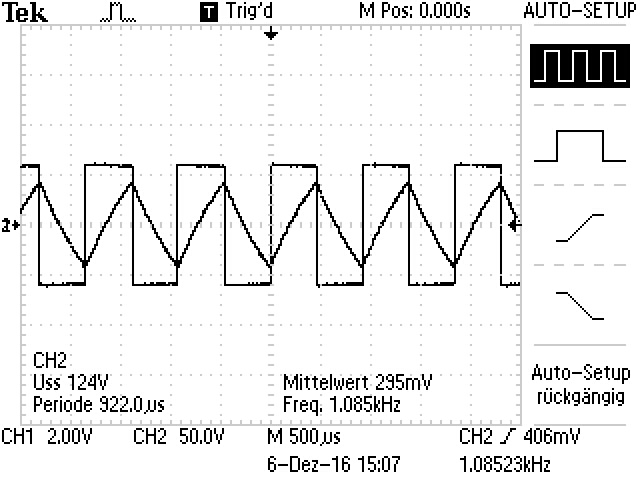
\includegraphics[width=0.98\textwidth]{bilder/ALL0001/F0001TEK.JPG}
		\label{fig:rorig}
	\end{subfigure}
\end{figure}
In Abbildung \ref{fig:rechteck} ist die Rechteckspannung sowie die über das RC-Glied integrierte Rechteckspannung dargestellt.
Die integrierte Rechteckspannung ist wie zu erwarten eine Dreiecksspannung.
\begin{figure}
	\caption{Aufgabenteil d: Sinusspannung}
	\label{fig:sinus}
	\centering
	\begin{subfigure}{0.48\textwidth}
		\centering
		\includegraphics[width=0.98\textwidth]{build/integration2.pdf}
		\label{fig:intsinus}
	\end{subfigure}
	\begin{subfigure}{0.48\textwidth}
		\centering
		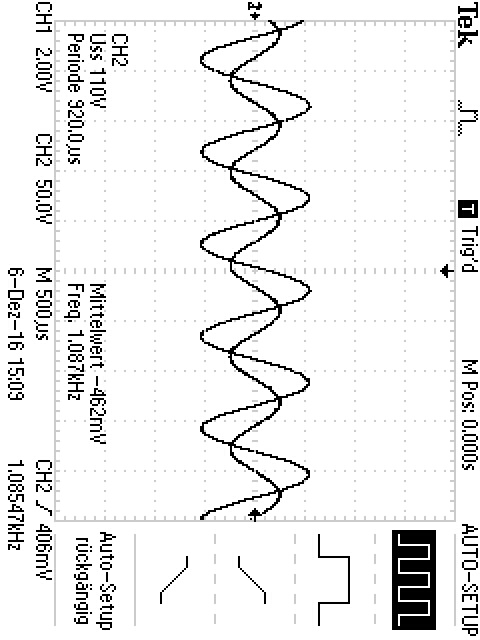
\includegraphics[width=0.98\textwidth]{bilder/ALL0002/F0002TEK.JPG}
		\label{fig:sorig}
	\end{subfigure}
\end{figure}

Der Spannungsverlauf der Sinusspannung ist in Abbildung \ref{fig:sinus} dargestellt. Wie zuvor ist die Kosinusspannung - integrierte Sinusspannung - außerdem in diesem Plot aufgezeichnet.

\begin{figure}
	\caption{Aufgabenteil d: Dreiecksspannung}
	\label{fig:dreieck}
	\centering
	\begin{subfigure}{0.48\textwidth}
		\centering
		\includegraphics[width=0.98\textwidth]{build/integration3.pdf}
		\label{fig:intdreieck}
	\end{subfigure}
	\begin{subfigure}{0.48\textwidth}
		\centering
		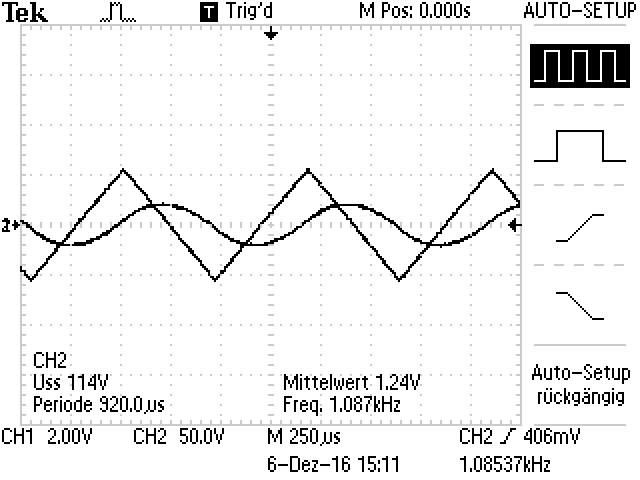
\includegraphics[width=0.98\textwidth]{bilder/ALL0003/F0003TEK.JPG}
		\label{fig:dorig}
	\end{subfigure}

\end{figure}

In Abbildung \ref{fig:dreieck} ist eine Dreieck- und die sich ergebende Parabelspannung aufgetragen.
